\documentclass[14pt, a4paper]{report}
\usepackage{mathtext}
\usepackage[T2A]{fontenc}
\usepackage[utf8]{inputenc}
\usepackage[russian]{babel}
\usepackage{multirow}
\usepackage{slashbox}
\usepackage{makecell}
\usepackage{graphicx}
\usepackage{physics}
\usepackage{amstext}
\usepackage{caption}
\usepackage{subcaption}
\usepackage{cmap}
\usepackage{float}

\renewcommand{\thesection}{\arabic{section}.}
\renewcommand{\thesubsection}{\arabic{section}.\arabic{subsection}.}

\title{\textbf{Отчет о выполнении лабораторной работы}}
\author{Калашников Михаил, Б03-202}
\date{}

\begin{document}
\maketitle

\textbf{Цель работы:}

\textbf{В работе используются:}
\begin{itemize}
\item
\end{itemize}

\section{Теоретические сведения}

\section{Экспериментальная установка}

\section{Проведение эксперимента}

\begin{enumerate}

\item Включим пересчетный прибор, высоковольтный выпрямитель и форвакуумный насос.

\item Дождемся откачки камеры спектрометра. Степень откачки будем измерять проводя измерения интенсивности $\beta$-излучения и отмечая уровень изменения показаний.

\item Приступим к измерению спектра. Будем повышать ток в катушке от 0 до 4.2 А с шагом 0.2 А. Каждое измерение длится 100 секунд. Получим следующий набор точек.

\begin{figure}[H]
\centering
\makebox[\textwidth][c]{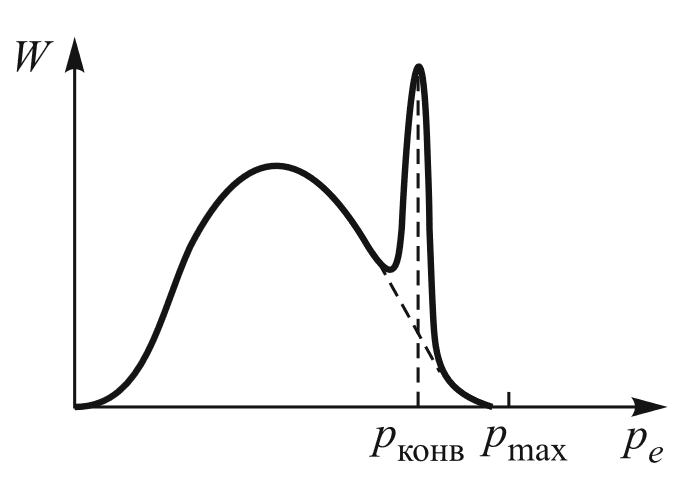
\includegraphics[scale=1]{../images/542-1}}
\caption{Первичное измерение спектра}
\end{figure}

\item Из полученных измерений можно сделать вывод что конверсионный пик лежит в диапазоне от 3 до 3.6 А. Проведем измерения данного участка с шагом 0.05 А. Из всех точек вычтем среднее значение первой и последней точек, приняв его за фоновое излучение ($N_{ф}=(0.92\pm0.15)\ с^{-1}$).

\begin{figure}[H]
\centering
\makebox[\textwidth][c]{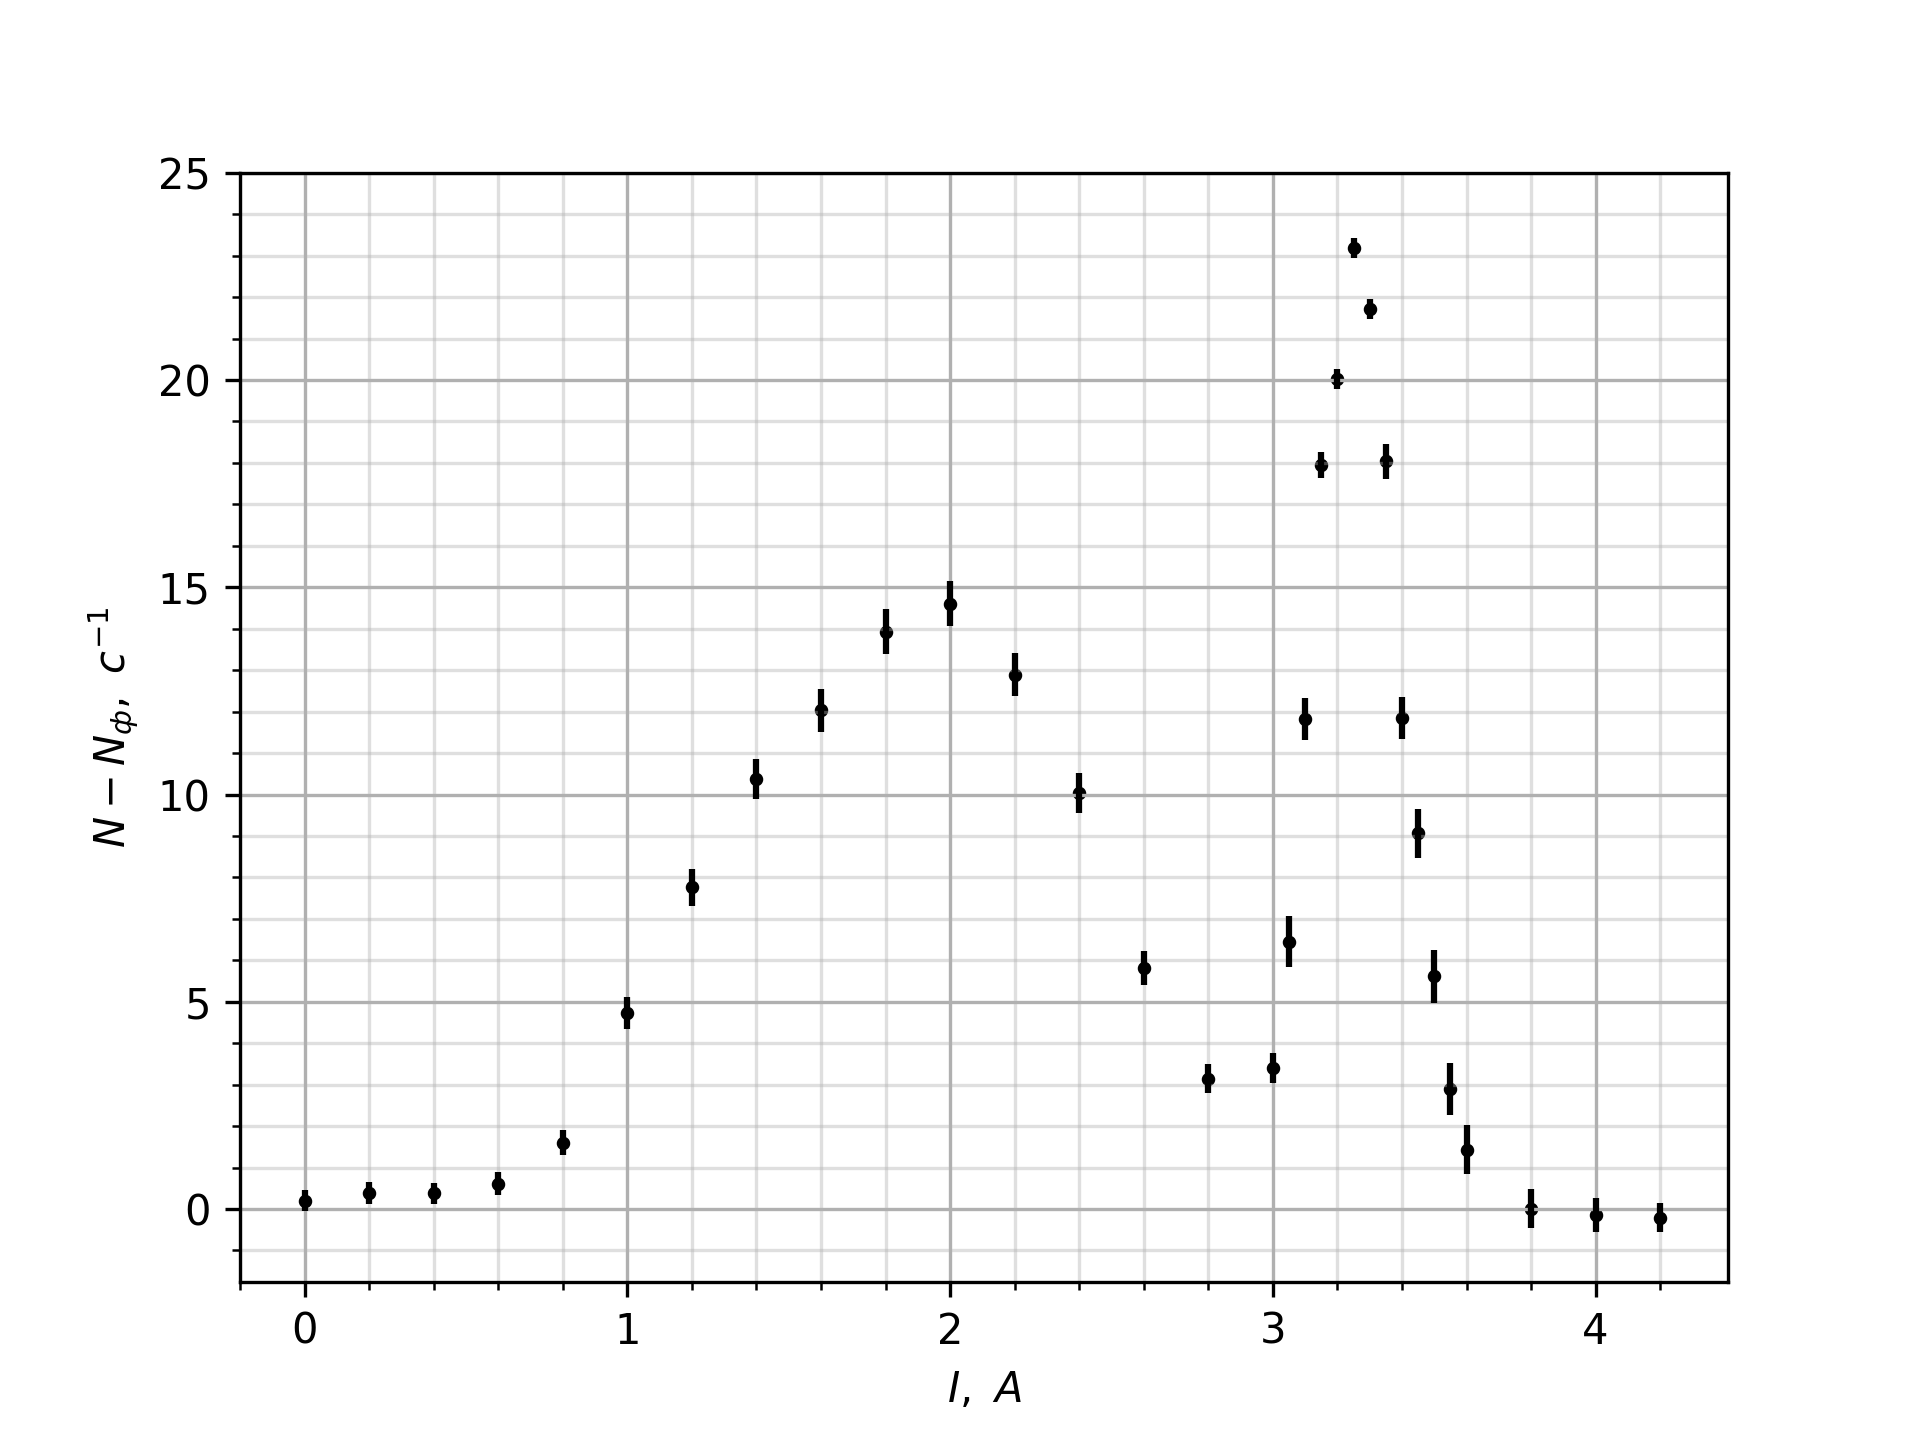
\includegraphics[scale=1]{../images/542-2}}
\caption{Измереный спектр $\beta$-излучения}
\end{figure}

\end{enumerate}

\section{Обработка результатов}

\begin{enumerate}

\item Проведем калибровку спектрометра. Для этого определим расположение конверсионного пика. Две точки пика с максимальными значениями расположены при 3.30 А и 3.35 А. Тогда точкой пика можно считать:

\[I_{конв}=(3.325\pm0.05)\ А\]

\item Зная, что $(pc)_{конв}=1013.5\ кэВ$, рассчитаем константу прибора:

\[k=\frac{(pc)_{конв}}{I_{конв}}=(305\pm5)\ \frac{кэВ}{А}\]

\item Теперь можем построить график Ферми. Зная, что спектр описывается формулой

\[\sqrt{\frac{N-N_{ф}}{p^3}}=a(T_{max}-T),\]

построим график в координатах $\sqrt{(N-N_{ф})/p^3}$ по оси ординат и $T$ по оси абсцисс.

\begin{figure}[H]
\centering
\makebox[\textwidth][c]{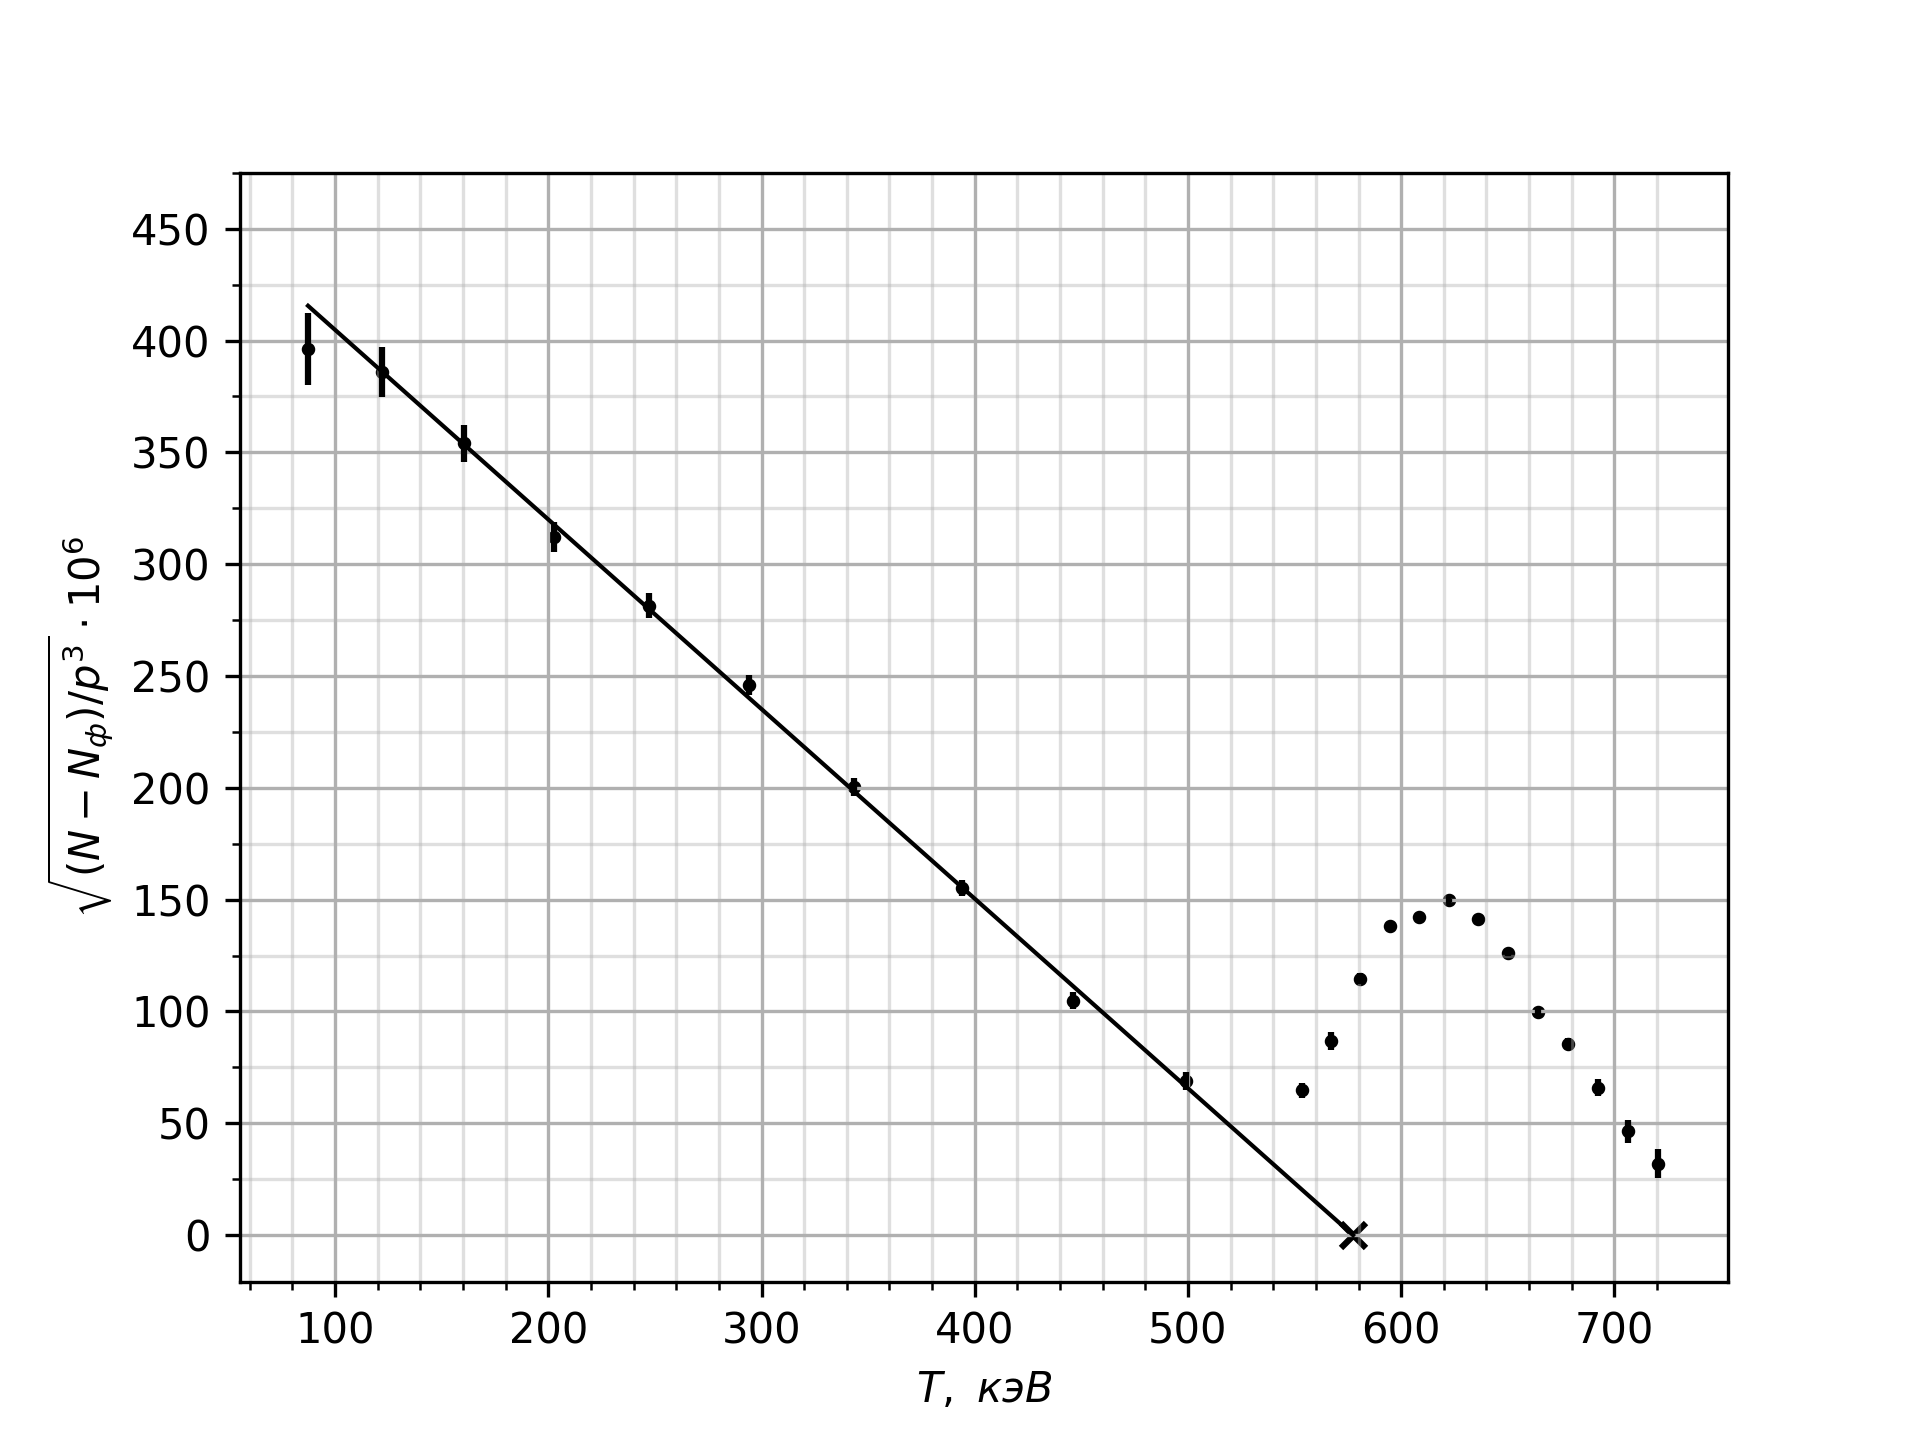
\includegraphics[scale=1]{../images/542-3}}
\caption{График Ферми}
\end{figure}

\item Через часть этих точек можно провести прямую. Точка пересечения этой прямой с осью абсцисс будет равна $T_{max}$:

\[T_{max}=(560\pm4)\ кэВ\]

\end{enumerate}

\section{Выводы}



\end{document}